\documentclass[12pt]{article}
\usepackage{graphicx}
\usepackage {color}
\usepackage{pdfpages}
\usepackage{float}
\usepackage{changebar}
\usepackage{enumitem,amssymb}
\renewcommand{\familydefault}{\sfdefault}
\usepackage[margin=1.2in]{geometry}
\usepackage{graphicx}
\usepackage{wrapfig}
\usepackage[super]{cite}
\usepackage{subcaption}
\usepackage[table]{xcolor}
\usepackage{amsmath}
\usepackage[sort, numbers]{natbib}
\usepackage{matlab-prettifier}
\usepackage{wrapfig,lipsum,booktabs}
%%%%%%%%%%%%Defining the margins %%%%%%%%%%%%%%%%%%%%%
\textheight 9.in
\textwidth 6.5in
\topmargin -.5in
\oddsidemargin 0in
\setlength{\parskip}{\smallskipamount}

%%%%%%%%%%%%%%Specific Commands %%%%%%%%%%%%%%%%%%
\newcommand{\eg}{{\em e.g.,}}
\newcommand{\ie}{{\em i.e.,}}
\newcommand{\etc}{{\em etc.,}}
\newcommand{\etal}{{\em et al.}}
\newcommand{\degrees}{{$^{\circ}$}}
\newcommand{\micro}{{$\mu$}}


%%%%%%%%%%%%%%%%%%%%%%%%%%%% Setting to control figure placement
% These determine the rules used to place floating objects like figures 
% They are only guides, but read the manual to see the effect of each.
\renewcommand{\topfraction}{.9}
\renewcommand{\bottomfraction}{.9}
\renewcommand{\textfraction}{.1}
\renewcommand{\familydefault}{\sfdefault} %setting the san serif font

%%%%%%%%%%%%%%%%%%%%%%%% Line spacing
% Use the following command for ``double'' spacing
%\setlength{\baselineskip}{1.2\baselineskip}
% and this one for an acceptable NIH spacing of 6lpi based on 11pt
%\setlength{\baselineskip}{.9\baselineskip}
% The baselineskip does not appear to work when we include a maketitle
% command in the main file.  Something there must set the line spacing
% If we use this next command, then things seem to work.
\renewcommand{\baselinestretch}{.9}

\setcounter{secnumdepth}{0} %make no numbers but have a table of contents


\begin{document}

\title{Lab 2, Propagation}
\author{Jake Bergquist, u6010393}
\maketitle
\tableofcontents
\newpage

\section{Introduction}
A single cardiac myocyte becomes activated when its resting membrane voltage is perturbed from roughly -80 mV to roughly -40 mV, the threshold potential for voltage sensitive sodium channels to open. At this point the sodium channels begin to open, causing a positive feedback of sodium channel activation and rise in membrane potential delineating the upstroke of the myocyte action potential. In isolation the initial current that causes the depolarization of the membrane to the action potential threshold is caused by some unknown or known stimulus, but in actual working myocardium or even cultured and simulated tissues this stimulus come from neighboring cardiomyocytes. Cardiomyocytes are linked to their neighbors by conductive channels called gap junctions that allow relatively free passage of ions (and therefore current) and water between the cells. Thus the depolarization and activation of one cardiomyocyte will cause depolarizing currents to pass through the gap junctions into neighboring cells, bringing their membrane potentials closer to threshold. In this way, activation of cardiomyocytes spreads or propagates from cell to cell. The speed, efficiency, and viability of this propagation is controlled by many physiological factors both on a cellular, tissue, and global scale.\cite{KLEBER2004} One of the key components is the conductivity of these gap junction channels. If the gap junctions are not conductive enough then neighboring cells will not receive sufficient stimulating current from activating cells to activate themselves. If the gap junctions are too conductive then the current flows too quickly from an activating cell, preventing it from reaching its threshold.

Modeling of cardiac electrophysiology allows to the examination of parameters and situations typically unavailable in experimental models.\cite{Fink2011} At a cellular level conductivities of individual channels can be modulated, ionic concentrations and stimulus protocols can be tightly controlled, and parameter measurements can be made at a level of detail and resolution that is impractical or impossible in experimental models.\cite{Sachse2008,TenTusscher2003} At the multicellular, tissue, and organ scale all of these benefits apply. Conduction between cells can be altered to investigate various disease states, and models can be tailored to match interesting physiological scenarios.\cite{Livshitz2009} Models can also be designed at varying levels of complexity and refinement to allow for coarser or finer investigation of various phenomena. In order to use a computational model to interrogate propagation there are two key components that must be considered. The simulation must incorporate both models at a cellular scale to describe how individual myocytes behave as well as some model to explain the coupling between the activity of myocytes and their neighbors. The former is needed to understand when a ``cell" in the model is excited and how it will behave, and the latter is needed to understand how this electrical activity during excitation can spread to neighboring myocytes. By constructing the simulation in this way researchers can examin the effects of both of these phenomena, the cellular and the connectivity between cells, and its effect of the resultant propagation.

One are of interest in understanding propagation is examining situations where it fails. When a wave of activity is spreading through a group of cells, be it as a single fiber, sheet, or 3D structure, the movement and propagation of the wavefront of activation can be thought of in terms of sources ans sinks. The source is the cells which are activating or have just been activated, those in the early phases of their action potentials. The sinks are the regions of tissue adjacent to the source that has not been activated yet, the cells whose membrane voltages are below threshold. Current flows from the cells in the source to those in the sink through gap junctions. When the source and sink are matched in size, or when the source is able to provide enough current then there is no problems and the activation front is able to propagate. However, consider the situation where a thin fiber of tissue is activated then connects to a larger area of tissue. At the boundary between the fiber and the lager area there is a relatively small source compared to the rapidly growing sink, resulting in a source sink mismatch in this direction of propagation, and therefore a potential for conduction failure. If the disparity between the source and sink is great enough, depending on the coupling of the cells the source will be unable to provide sufficient current to activate the sink. Source sink mismatch, however, does not occur in the reverse direction because the source of the larger area of tissue is much greater and able to provide sufficient current to activate the small fiber. This then creates the ideal scenarios fo a unidirectional conduction block whereby the propagation is able to progress in only one direction. The geometry of the tissue is not the only factor that can affect source-sink matching. Tissue which is damaged or experiencing an insult such as myocardial ischmia can display conduction abnormalities preventing that tissue from performing adequately as a source, resulting again in potential unidirectional blocks. These unidirectional blocks are problematic in that they can set up conditions within the tissue for arrhythmogenesis and sustaining of arrhythmias, which can be fatal.

Given the importance of understanding when conduction will be successful and when it might fail, a useful parameter can be examined called the safety factor. It is defined as the ratio between charge generated during activation and the amount of charge consumed during the activation process. For example, a single cell in a chain of connected myocytes may generate N charge during its activation, and as this activation spreads to the neighboring cell, 0.5N of that charge is consumed by current flowing to the other cell (as well as capacitive and resistive loss). Thus the safety factor in this case would be 2. When the safety factor falls below 1 then there is a porpagation failure due to insufficient charge being generated to continue the activation.

\section{Methods}
\begin{wraptable}{r}{5.5cm}
	
	\centering
	\caption{Simulation parameters for the 17 examined simulations}
	\begin{tabular}{|l|l|l|l|}
		\hline
		Simulation & I$_{stim}$& Coupling & I$_{Na}$  \\ 
		&    $\mu A/\mu F$   & $cm^2/ms$         & Scale     \\ \hline
		1          & 120   & 7e-5     & 1    \\ \hline
		2          & 120   & 1e-4     & 1    \\ \hline
		3          & 120   & 2e-4     & 1    \\ \hline
		4          & 120   & 7e-4     & 1    \\ \hline
		5          & 120   & 1e-3     & 1    \\ \hline
		6          & 120   & 2e-3     & 1    \\ \hline
		7          & 120   & 3e-3     & 1    \\ \hline
		8          & 110   & 7e-4     & 1    \\ \hline
		9          & 100   & 7e-4     & 1    \\ \hline
		10         & 90    & 7e-4     & 1    \\ \hline
		11         & 80    & 7e-4     & 1    \\ \hline
		12         & 120   & 7e-4     & 2    \\ \hline
		13         & 120   & 7e-4     & 0.75 \\ \hline
		14         & 120   & 7e-4     & 0.5  \\ \hline
		15         & 120   & 7e-4     & 0.4  \\ \hline
		16         & 120   & 7e-4     & 0.3  \\ \hline
		17         & 120   & 7e-4     & 0.25 \\ \hline
	\end{tabular}
\label{tab:params}
\end{wraptable}
The software used is a series of matlab functions and scripts to utilize the myocyte electrophysiology model developed by Luo-Ruy (1991) to simulate propagation in a single cell chain of connected myocytes. The conduction model implementation was developed by Livshitz and Rudy in 2009.\cite{Livshitz2009} The main function driving the simulation (main\_LRd\_strand.m) takes in a structure array contiaining the parameters of Istim (the stimulus current), coupling (the coupling constant representitive of the gap junctions between the cells), and INaScale (the scaling of the sodium conductance withint he Luo-Rudy cell model). By varying these parameters one can visualize their effect based on plotted action pointials in time and space, as well as intepret the calculated conduction velocity along the fiber and the maximum upstroke of the action potential. I have designed a wrapper script to iterate through the parameters of interest for 17 simulations listed in Table~\ref{tab:params}. This wrapper script leverages the paralell computing toolbox to fun all of the simulations in paralell on the CPU, dramatically decreasing the run time of the simulations. Unfortunately, plotting of figures is difficult during paralell computation in Matlab, thus I have modified the original main\_LRd\_strand function to also output the transmembrane potentials in order to plot them in a separate loop. The transmembrane potentials are already calculated int he original main function, I simply added them as an output variable. Below is the matlab script I developed and the associated function for running the simulations for this lab.

\begin{lstlisting}[style=Matlab-editor]
%Lab 2 Driving Script
%Author: Jake Bergquist
%2019
clear
close all
clc
%Simulation parameters:
simParams=[120,120,120,120,120,120,120,110,100,...
	90,80,120,120,120,120,120,120;...
	7e-5,1e-4,2e-4,7e-4,1e-3,2e-3,...
	3e-3,7e-4,7e-4,7e-4,7e-4,7e-4,...
	7e-4,7e-4,7e-4,7e-4,7e-4;...
	1, 1, 1, 1, 1, 1, 1, 1, 1, 1, 1, 2,...
	 0.75, 0.5, 0.4, 0.3, 0.25]';


%Preallocate for speed
CV{length(simParams)} = [];
dVdtMax{length(simParams)} = [];
TMPs{length(simParams)}=[];
parfor ind = 1:length(simParams)
% set parameters
figure(ind);plot(rand(25));drawnow();
fprintf(sprintf('Setting Parameter Set %d\n',ind));
%Function defined below
Pstruct = setPstruct(simParams(ind,:));

% run the simulation
fprintf(sprintf('Running Simulation for Parameter Set %d\n',ind));
%The original function was modified 
%to also pass the TMP values for
%plotting later
[CV{ind}, dVdtMax{ind},TMPs{ind}]=main_LRd_strand(Pstruct, 2);
fprintf(sprintf('Finished Simulation For Parameter Set %d\n',ind));

end
%%

%The plot functionality was pulled 
%out of the original function in order to
%levarage parfor while also 
%plotting everything. To do so the following
%variables were also pulled out

Time = 200; N = 1;Tmesh=800;
tp=linspace(0,Time*N,Tmesh*N);
Xsize=1;Xmesh=50;%% 1 cm=100 cells; default Xmesh: 50
x = linspace(0,Xsize,Xmesh);
[Xp,Tp]=meshgrid(tp,x);
counter1 = 0;
counter2 = 0;

for ind = 1:length(simParams)

figure(ind);clf();
h=mesh(Tp',Xp',TMPs{ind});
ylabel(['Time [ms]'])
xlabel(['Fiber [cm]'])
view(-37,70)
zlabel('V_m (mV)')
axis tight
box off
grid off
set(gca,'fontsize',18)
view(80,30);%set desired view
%These specific movegui parameters 
%are set for my monitor, and may need
%adjustment to be compatible. 
%The next line could also be omitted
movegui(figure(ind),[560*counter1,420*counter2]);
counter1=counter1+1;
if mod(ind,5) == 0
counter2 = counter2+1;
counter1 = 0;

end

title(ind)

end


function Pstruct = setPstruct(simParams)
%This function is added to set 
%the parameters for the simulation withint he
%paralell loop. Setting struct values
% is tricky in a parfor loop thus this
%function was necessitated to hide 
%the assignment from the parfor


Pstruct.Istim = simParams(1);
Pstruct.coupling = simParams(2);
Pstruct.INaScale = simParams(3);

end


\end{lstlisting}

\section{Results}
\begin{wraptable}{r}{5.5cm}
	
	\centering
	\caption{Simulation results for 17 parameter sets.}
	
	\begin{tabular}{|l|l|l|}
		\hline
		Simulation & C.V.   & M.U.V.  \\ 
		& (cm/s) & (V/s)   \\ \hline
		1          & 16.6   & 69.9    \\ \hline
		2          & 19.0   & 73.9    \\ \hline
		3          & 24.7   & 83.87   \\ \hline
		4          & 45.3   & 109     \\ \hline
		5          & 52.6   & 117     \\ \hline
		6          & 77.6   & 132     \\ \hline
		7          & 2.06   & 0.0222  \\ \hline
		8          & 44.1   & 109     \\ \hline
		9          & 45.3   & 109     \\ \hline
		10         & 2.10   & -0.0024 \\ \hline
		11         & 2.10   & -0.0024 \\ \hline
		12         & 60.4   & 179     \\ \hline
		13         & 38.8   & 86.9    \\ \hline
		14         & 32.0   & 60.7    \\ \hline
		15         & 27.6   & 48.7    \\ \hline
		16         & 23.3   & 35.5    \\ \hline
		17         & 20.4   & 28.1    \\ \hline
	\end{tabular}
	\label{tab:r1}
\end{wraptable}
The numerical results for the 17 simulations tabulating the calculated conduction velocities (C.V.) and maximum upstroke velocities (M.U.V.) are listed in Table~\ref{tab:r1}. There are three main parameter maipulations to consider. Simulations 1-7 changed the coupling between the cells, and it can be observed that as the oupling increased the conduction velocity also increased to a point. However at simulation 7 where the coupling is at its maximum for these simulations the conduction velocity and upstrove velocity drop off. This is likely indicative of a failure of propagation. This theory is confirmed in Figure~\ref{fig:r1} where we can see the resulting action potentials from four of the 7 initial parameters. We see in simulation 7 (Figure~\ref{fig:r1}.D) there is only a stimulus resulting in a transmembrane voltage change ina  few of the cells that barely reaches -50 mV, not surpassing the required -40 mV threshold. We can also note the changes in conduction velocity betweent he different simulations as seen in Figure~\ref{fig:r1} by looking at the relative times at which the final action potentials initiate. As can be seen the simulation 1 shown in A has the final action potential initiate around 50 ms into the simulation, whereas for simulation 3 with an increased coupling the final action potential starts at around 25 ms. This indicates a clear increase in conduction velocity between the two reflected in Table~\ref{tab:r1}. However, what can also be seen is a decrease in action potential peak voltage in Figure~\ref{fig:r1}. This is related to the fact that with less coupling, more of the charge from activation stays within a cell and is not consumed by the neighboring cell activating, resulting in a higher peak voltage at the upstroke and as a result likely a larger safety factor. The increase in upstroke velocity as we increase coupling is due to the fact that at higher coupling, current can more readily flow into the next cell to be activated, activating it more rapidly. A slow activation leads to incomplete sodium channel recruitment and less steep upstroke, as seen in the reduced coupling cases.



\begin{figure}[H]
	\centering
	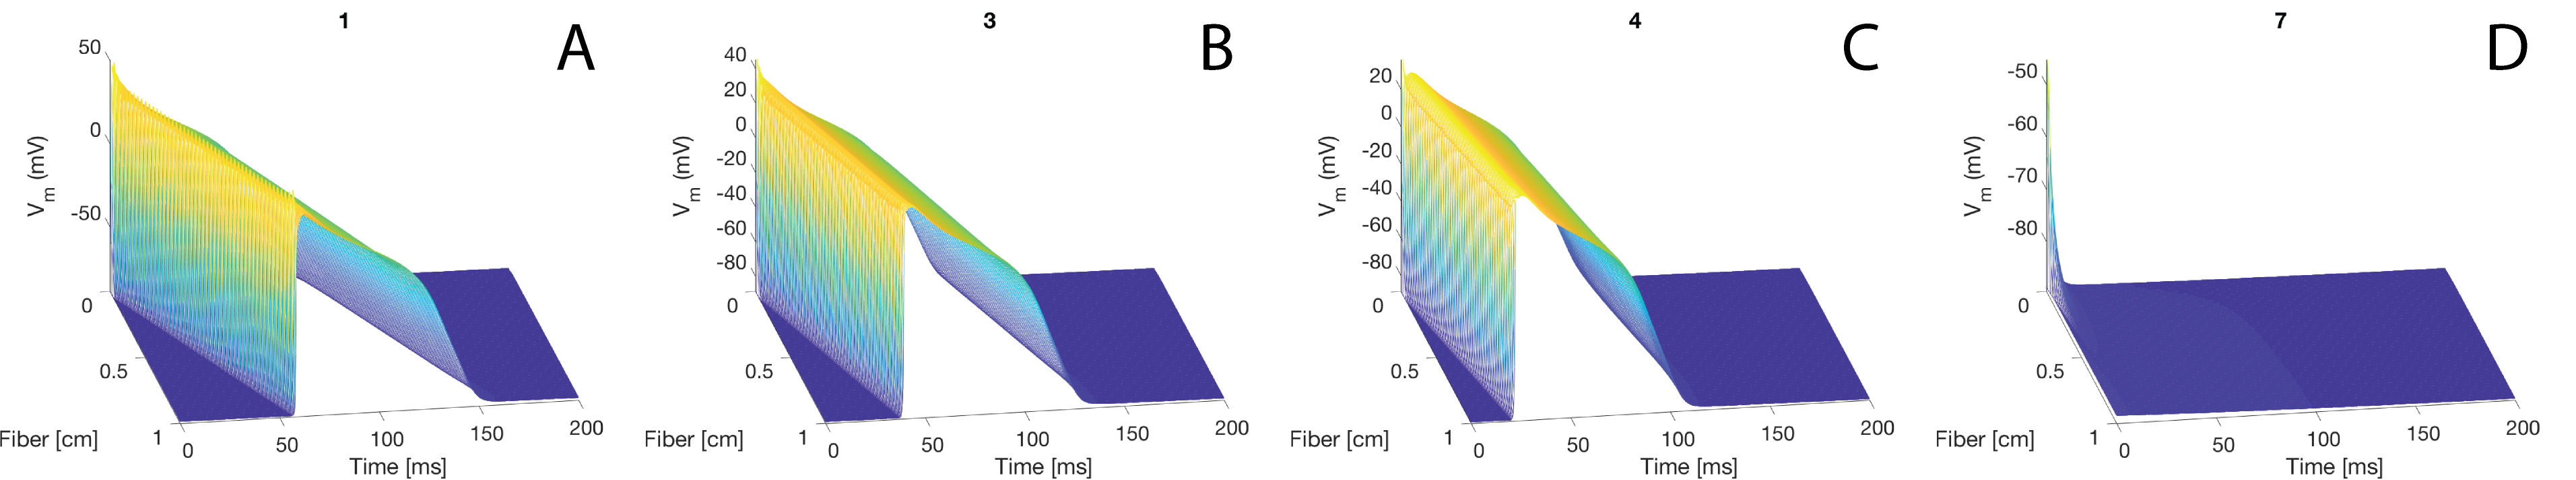
\includegraphics[width=\textwidth]{Figures/Fig1.png}
	\caption{A representitive selection of simulation results for the action potentials from the model. This subset examines the changes resulting from altered coupling between cells. A shows simulation 1, B shows simulation 3, C shows simulation 4, and D shows simulation 7.}
	\label{fig:r1}
\end{figure}

Simulations 4, 8, 9, 10, and 11 make up a parameter sweep over different stimulation currents. As would be expected the stimulation current does not effect the conduction velocity or upstroke velocity until the stimulus become insufficient to initiate an action potential in the first cell (Figure~\ref{fig:r2},Table~\ref{fig:r1}). This can be seen to occur at simulation 10 where the stimulation current falls to 90 $\mu A/\mu F$. Below this current with the given coupling and $I_{Na}$ scale, the Luo-Rudy cell model will not reach threshold potential, as can be seen in Figure~\ref{fig:r2}.D where the cells a the stimulus site only reach a membrane voltage of around -50 mV.

\begin{figure}[H]
	\centering
	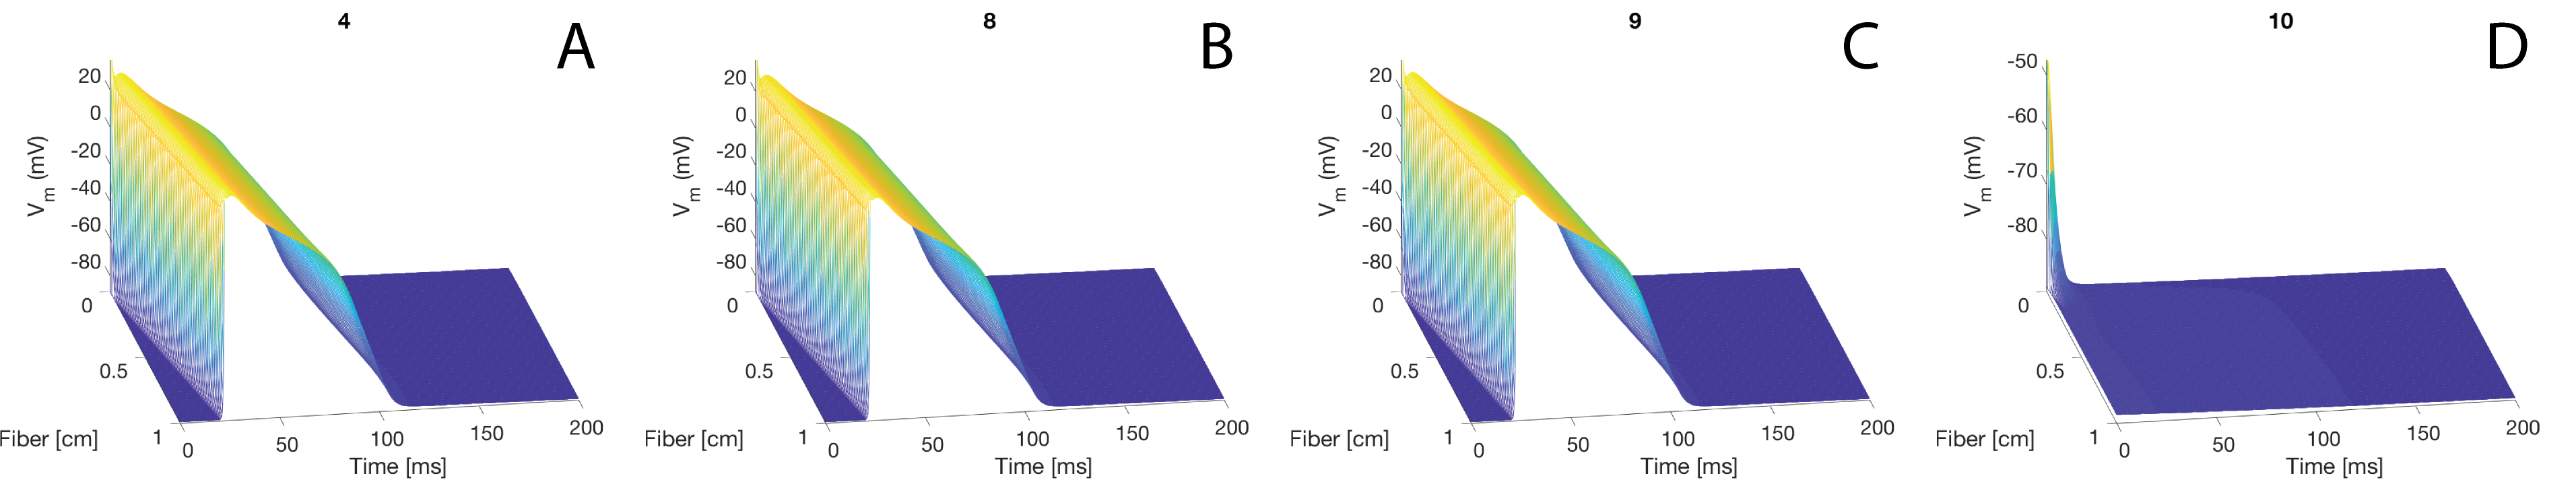
\includegraphics[width=\textwidth]{Figures/Fig2.png}
	\caption{A representitive selection of simulation results for the action potentials from the model. This subset examines the changes resulting from altered stimulation current. A shows simulation 4, B shows simulation 8, C shows simulation 9, and D shows simulation 10.}
	\label{fig:r2}
\end{figure}

Finally simulations 4, 12, 13, 14, 15, 16, and 17 make up a parameter sweep of different $I_{Na}$ scales. Changes in the $I_{Na}$ scale affect the conductivity of the sodium channel in the Luo-Rudy model once the cell has been activated. As the $I_{Na}$ scale decreased the conduction velocity also decreased as well as the upstroke velocity, however when compared tot he similar results seen in the coupling changes simulations (1-7) the changes to upstroke velocity are much more drastic while the changes to conduction velocity are less dramatic. Changes in $I_{Na}$ scale also affect the shape of the action potentials, particularly the upstroke as seen in Figure~\ref{fig:r3}. At elevated $I_{Na}$ scale (Figure~\ref{fig:r3}.A) the action potentials are sharper (higher upstroke velocity) and the peak voltage is higher, and as $I_{Na}$ scale decreases so too does the sharpness of the upstroke (Figure~\ref{fig:r3}.B-D). This contrasts with Figure~\ref{fig:r1} where conduction velocity also slowed as coupling decreased, but the action potential morphology was not as severely affected.

\begin{figure}[H]
	\centering
	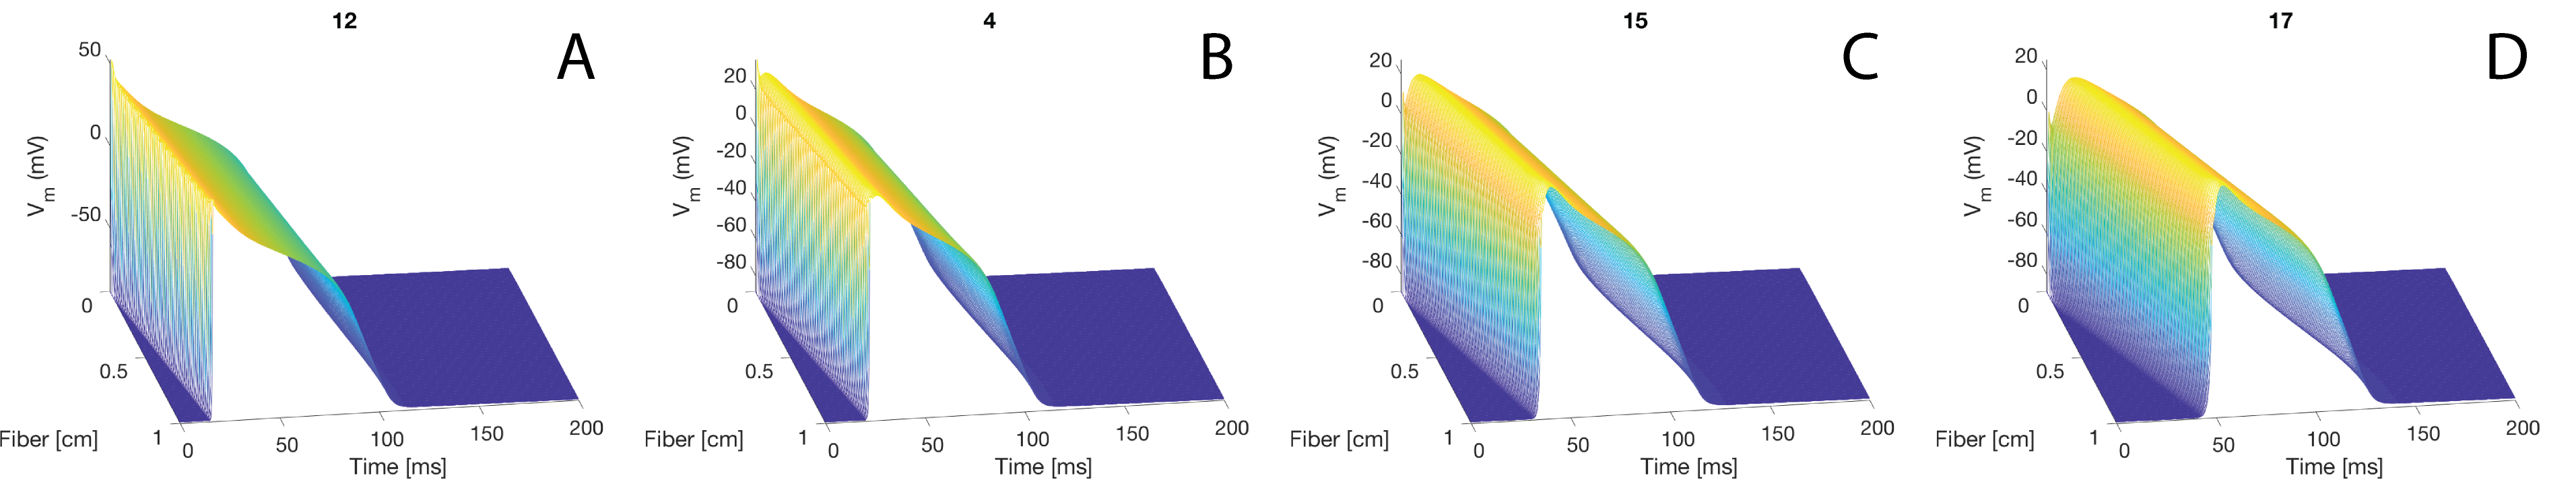
\includegraphics[width=\textwidth]{Figures/Fig3.png}
	\caption{A representitive selection of simulation results for the action potentials from the model. This subset examines the changes resulting from altered stimulation current. A shows simulation  12, B shows simulation 4, C shows simulation 15, and D shows simulation 17.}
	\label{fig:r3}
\end{figure}
\section{Discussion}
There are many parameters that affect conduction velocity and propagation in tissue. This model has allowed us to examine the effects of changes to cell to cell coupling, stimulation current, and changes to cellular physiology (in the form here of changes to sodium channel conductance). The clearest conclusion to draw is that changes in stimulation current to not drastically alter propagation in this model so long as the stimulus current is sufficient to incite an action potential by bringing the initial cell past its threshold voltage. 

The next interesting comparison is the changes caused by coupling alterations as compared to sodium channel changes. Decreasing cell-to-cell coupling in this model resulted in slower conduction velocity, as expected, given that with lower coupling it takes longer for a neighboring cell to be activated by the current hat is flowing to it from the previous activated cell. In the simple passive circuitry model it simply takes longer for the next cell to reach a certain voltage because the resistor between it and its charging ource (the previous cell) has increased in resistance. Compounding this over many cells leads to noticeable conduction velocity decreases. In the case that coupling goes too high there is a block in conduction because no cell can charge up to tis threshold voltage before that current leaks into the neighbor cell. In this case the safety factor is below 1, and we can observe this in Figure~\ref{fig:r1} where the stimulus current spreads rapidly into the first few cells, not fully depolarizing any of them to their threshold voltage. In the case of changes to $I_{Na}$ scale, reduction in the $I_{Na}$ scale also results in conduction velocity slowing. This makes sense given that  at lower sodium channel conductivity the amount of charge generated during the action potential is reduced, resulting in a decreased gradient of potential between the activated cell and the neighboring sink cell. This reduced gradient of potential results in a reduced magnitude of current between the two, thus a slower charging of the next cell to its activation threshold. This is observed in Figure~\ref{fig:r3}.B-D where the action potentials become less steep, and in Table~\ref{tab:r1} where the upstroke velocities decrease. The shape of the action potential is also affected as $I_{Na}$ scale changes, which contrasts changes to coupling that had minimal affect on action potential morphology other than changing peak voltage. When $I_{Na}$ scale is reduced the peak of the action potential is smoothed. This makes sense given the reduced conductivity of the sodium channels resulting a more sluggish upstroke before inactivating. Changes to action potential morphology can often be indicative of disease states of the myocytes themselves.

In real tissue there are more than just single lines of cells connected only at their ends. Cells are arranged in fibers and sheets in a complex 3D arrangement where any given myocyte is surrounded by neighbors to which it is connected by gap junctions. While most of the connections occur at the terminal ends of the myocyte there are also flanking connections to the myocytes that surround the sides of a given myocyte. As pointed out by Rohr et. al, this has the effect of smoothing and averaging local discontinuities in conduction.\cite{Rohr2004} Additionally in the context of source sink relationships often there is not just one cell trying to propagate an activation to another, but rather there are hundreds and thousands of cells activated that are the sources for a sink that is made up also of hundred and thousands of cells. There are some special cases (purkinje-myocardial junctions) that exhibit the classic scenario expected of source sink mismatch with the source being small and sink being large. However, in these cases the purkinje fibers are able to activate the myocardium. Perhaps this is by cooperative activity of many fibers, perhaps by changes in coupling between the fibers and the tissue. Rohr et. al described a scenario where reducing coupling to a degree could solve such a source sink mismatch, perhaps by allowing the smaller source to have a relatively smaller sink to interact with by way of reduced coupling to the larger volume of the sink.\cite{Rohr2004} In the context of safety factor of conduction, the 3D structure and interconnected nature of real tissue is both beneficial and detremental. While there is a larger amount of charge consumed during the activation of a large sink, there is also a larger source to provide that charge. The result is that overall the longitudinal and transverse connections between myocytes allows for a more homogeneous activation which is more coordinated, thereby minimizing the chance of encountering a source sink mismatch where the safety factor would fall close to or below 1. In this way the healthy heart guarantees propagation.
%%%%%%%%%%%%%%%%%% Correct Bibliography Style

\bibliography{/Users/jbergquist/Documents/BibTex/Library}
\bibliographystyle{ieeetr}


\end{document}








